\documentclass{beamer}

%% Juego de caracteres usado en el archivo fuente: UTF-8
\usepackage{ucs}
\usepackage[utf8x]{inputenc}
\uselanguage{spanish}
%Para la identación del español
\usepackage[spanish]{babel}

% There are many different themes available for Beamer. A comprehensive
% list with examples is given here:
% http://deic.uab.es/~iblanes/beamer_gallery/index_by_theme.html
% You can uncomment the themes below if you would like to use a different
% one:
%\usetheme{AnnArbor}
%\usetheme{Antibes}
%\usetheme{Bergen}
%\usetheme{Berkeley}
%\usetheme{Berlin}
%\usetheme{Boadilla}
%\usetheme{boxes}
%\usetheme{CambridgeUS}
%\usetheme{Copenhagen}
%\usetheme{Darmstadt}
%\usetheme{default}
%\usetheme{Frankfurt}
%\usetheme{Goettingen}
%\usetheme{Hannover}
%\usetheme{Ilmenau}
%\usetheme{JuanLesPins}
%\usetheme{Luebeck}
\usetheme{Madrid}
%\usetheme{Malmoe}
%\usetheme{Marburg}
%\usetheme{Montpellier}
%\usetheme{PaloAlto}
%\usetheme{Pittsburgh}
%\usetheme{Rochester}
%\usetheme{Singapore}
%\usetheme{Szeged}
%\usetheme{Warsaw}

%Para la identación del español
\usepackage[spanish]{babel}

\title{Ofertas Steam Mule}

% A subtitle is optional and this may be deleted
%\subtitle{Optional Subtitle}

\author{Jesús Rodríguez Heras \\ Juan Pedro Rodríguez Gracia}
% - Give the names in the same order as the appear in the paper.
% - Use the \inst{?} command only if the authors have different
%   affiliation.

%\institute[Escuela Superior de Ingeniería] % (optional, but mostly needed)
%{
%  \inst{1}%
%  Department of Computer Science\\
%  University of Somewhere
%  \and
%  \inst{2}%
%  Department of Theoretical Philosophy\\
%  University of Elsewhere}
% - Use the \inst command only if there are several affiliations.
% - Keep it simple, no one is interested in your street address.

\date{25 de abril de 2018}
% - Either use conference name or its abbreviation.
% - Not really informative to the audience, more for people (including
%   yourself) who are reading the slides online

%\subject{Theoretical Computer Science}
% This is only inserted into the PDF information catalog. Can be left
% out. 

% If you have a file called "university-logo-filename.xxx", where xxx
% is a graphic format that can be processed by latex or pdflatex,
% resp., then you can add a logo as follows:

% pgfdeclareimage[height=0.5cm]{university-logo}{university-logo-filename}
% \logo{\pgfuseimage{university-logo}}

% Delete this, if you do not want the table of contents to pop up at
% the beginning of each subsection:
%\AtBeginSubsection[]
%{
%  \begin{frame}<beamer>{Índice}
%    \tableofcontents[currentsection,currentsubsection]
%  \end{frame}
%}

% Let's get started
\begin{document}

\begin{frame}
  \titlepage
  
\end{frame}

\begin{frame}{Índice}
  \tableofcontents
  % You might wish to add the option [pausesections]
\end{frame}

% Section and subsections will appear in the presentation overview
% and table of contents.

\section{Esquema de flujo}
\begin{frame}{Esquema de flujo}
	\begin{center}
		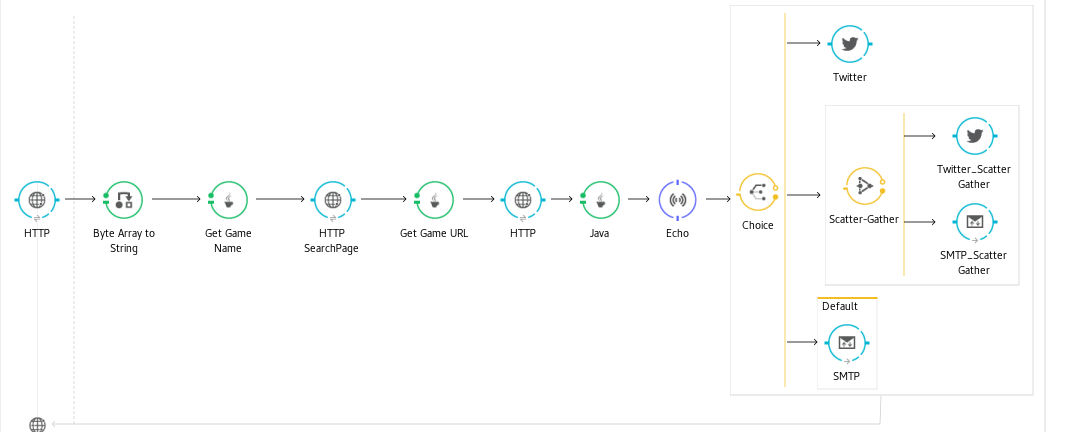
\includegraphics[scale=0.45]{diagrama2.png}
	\end{center}
\end{frame}

\section{Funcionamiento}
\begin{frame}{Funcionamiento}
	\begin{block}{¿Cómo funciona?}
		Para lanzar la aplicación, el usuario debe abrir su navegador e introducir la siguiente dirección en la barra de direcciones:\\
		\url{localhost:8081/game/nombreJuego}\\
		Siendo \texttt{nombreJuego} el nombre del juego que queremos buscar.
	\end{block}
	\begin{exampleblock}{Por ejemplo}
		\url{localhost:8081/game/rocket\%20league}
	\end{exampleblock}
\end{frame}

\begin{frame}{Funcionamiento}
	\begin{enumerate}
		\item El usuario introduce la url con el nombre del juego.
		\item Mediante la clase \texttt{GetNombre.java} eliminamos toda la url excepto el nombre del juego.
		\item Introducimos el nombre del juego en el buscador de Steam.
		\item El ESB accede a la página de la búsqueda de Steam y devuelve el código html de la página a la clase \texttt{GetGamePage.java}, la cual busca la url de la primera ocurrencia del buscador.
		\item Entramos en la paǵina y buscamos el precio mediante la clase \texttt{GetGameOffer.java}.
		\item Ahora comprobamos si el juego está en oferta o no.
		\begin{enumerate}
			\item Sin oferta.
			\item En oferta.
			\item +18.
			\item ``Free to Play''.
			\item No existe el juego.
		\end{enumerate}
	\end{enumerate}
\end{frame}

\section{Resultados}
\begin{frame}{Veamos los resultados}
	\begin{block}{Resultados}
		\begin{itemize}
			\item Si entramos en el correo electrónico, podremos ver los juegos que han sido buscados por el usuario con sus respectivos precios.
			\item Si entramos en la cuenta de twitter \href{https://twitter.com/MuleSteam}{\texttt{\textit{@MuleSteam}}}, podremos ver las ofertas que se han ido publicando por el sistema.
		\end{itemize}
	\end{block}
\end{frame}

\section{Problemas encontrados}
\begin{frame}{Problemas encontrados}
	\begin{alertblock}{Hemos encontrado los siguientes problemas}
		\begin{itemize}
			\item Correo en el dominio de google.
			\item Mayores de edad.
			\item Free to Play.
			\item No existe el juego.
			\item Problemas menores con la \href{https://help.twitter.com/en/rules-and-policies/twitter-automation}{\textit{política de spam de twitter}}.
		\end{itemize}
	\end{alertblock}
\end{frame}

\section{¿Preguntas?}
\begin{frame}{¿Preguntas?}
\begin{center}
	
\includegraphics[scale=1.3]{dudasTumbado.jpg}
\end{center}

\end{frame}

\end{document}


